\documentclass[12pt,a4paper]{article}
\usepackage[utf8]{inputenc}
\usepackage{ctex} % 支持中文
\usepackage{amsmath, amssymb, amsthm}
\usepackage{graphicx}
\usepackage{listings}
\usepackage{xcolor}
\usepackage{tabularx}
\usepackage{booktabs}
\usepackage{float} % Required for the H float option

\lstset{
    language=Python, % 添加语言支持
    basicstyle=\ttfamily\small,
    numbers=left,
    numberstyle=\tiny,
    keywordstyle=\color{blue},
    commentstyle=\color{gray},
    stringstyle=\color{red},
    breaklines=true,
    frame=single,
    captionpos=b
}

\title{计算流体力学作业5}
\author{郑恒2200011086}
\date{\today}

\begin{document}

\maketitle

\section{问题介绍}
在单位正方形内,求解不可压缩流动。仅上边界为水平运动边界,其余边界均为固定壁面。上边界速度分布设为
\[
u(x) = \sin^2(\pi x)
\]
该分布在角点处函数值和导数均为零,保证了速度场的连续性。通过数值方法计算流场,考察不同位置的速度剖面、主涡涡心位置和流函数值等。使用Python语言,设运动粘度$\nu=0.001$,画出流线图,并对主要物理量进行讨论。

\section{算法原理}
对于不可压缩流体,流场满足的方程为Navier-Stokes方程。对于二维不可压缩流体,Navier-Stokes方程可以写成如下形式:
\begin{equation}
    \frac{\partial u}{\partial t} + u \frac{\partial u}{\partial x} + v \frac{\partial u}{\partial y} = -\frac{1}{\rho} \frac{\partial p}{\partial x} + \nu \left( \frac{\partial^2 u}{\partial x^2} + \frac{\partial^2 u}{\partial y^2} \right)
\end{equation}
\begin{equation}
    \frac{\partial v}{\partial t} + u \frac{\partial v}{\partial x} + v \frac{\partial v}{\partial y} = -\frac{1}{\rho} \frac{\partial p}{\partial y} + \nu \left( \frac{\partial^2 v}{\partial x^2} + \frac{\partial^2 v}{\partial y^2} \right)
\end{equation}
\begin{equation}
    \frac{\partial u}{\partial x} + \frac{\partial v}{\partial y} = 0
\end{equation}
其中,$u$和$v$分别是流体在$x$和$y$方向的速度分量,$\rho$是流体密度,$p$是压力,$\nu$是运动粘度。
在本问题中,我们需要求解流体的速度场和压力场。我们使用有限差分法来离散化Navier-Stokes方程,并使用迭代方法来求解离散方程。
我们将流场离散化为一个网格,并在每个网格点上计算速度和压力。我们可以使用显式时间步进方法来更新速度和压力场。具体步骤如下:
\begin{enumerate}
    \item 初始化网格和边界条件
    \item 计算速度场和压力场
    \item 更新速度场和压力场
    \item 重复步骤2和3,直到收敛
    \item 计算主涡涡心位置和流函数值
    \item 绘制流线图和速度剖面
    \item 输出结果
\end{enumerate}

在本问题中,密度$\rho$被视为常数,不随空间和时间变化。由于$\rho$为常数,实际计算时常常将其归一化处理,即令$\rho=1$,以简化方程和计算。

在迭代计算速度场合压力场时,我们采用投影法,以下是投影法的步骤公式:
\begin{enumerate}
    \item 预测步:先不考虑压力项,计算临时速度场$\mathbf{u}^*$:
    \begin{equation}
        \frac{\mathbf{u}^* - \mathbf{u}^n}{\Delta t} = -(\mathbf{u}^n \cdot \nabla)\mathbf{u}^n + \nu \nabla^2 \mathbf{u}^n
    \end{equation}
    其中,$\mathbf{u}^n$为当前时刻速度,$\mathbf{u}^*$为预测速度。

    \item 压力泊松方程:为保证不可压缩性,对预测速度场求解压力修正:
    \begin{equation}
        \nabla^2 p^{n+1} = \frac{1}{\Delta t} \nabla \cdot \mathbf{u}^*
    \end{equation}

    \item 修正步:用新压力修正速度场,得到下一个时刻的速度:
    \begin{equation}
        \mathbf{u}^{n+1} = \mathbf{u}^* - \Delta t \nabla p^{n+1}
    \end{equation}
    这样可以保证$\nabla \cdot \mathbf{u}^{n+1} = 0$,满足不可压缩条件。
\end{enumerate}

在实际算法中,我们需要对投影法的每一步进行离散化。
对于上述投影法的三个步骤,采用中心差分离散化,差分格式如下:

\begin{enumerate}
    \item 预测步:
    \begin{align}
        \frac{u^*_{i,j} - u^n_{i,j}}{\Delta t} = 
        &- u^n_{i,j} \frac{u^n_{i+1,j} - u^n_{i-1,j}}{2\Delta x}
        - v^n_{i,j} \frac{u^n_{i,j+1} - u^n_{i,j-1}}{2\Delta y} \notag \\
        &+ \nu \left(
            \frac{u^n_{i+1,j} - 2u^n_{i,j} + u^n_{i-1,j}}{\Delta x^2}
            + \frac{u^n_{i,j+1} - 2u^n_{i,j} + u^n_{i,j-1}}{\Delta y^2}
        \right)
    \end{align}
    对$v$分量同理。

    \item 压力泊松方程:
    \begin{equation}
        \frac{p^{n+1}_{i+1,j} - 2p^{n+1}_{i,j} + p^{n+1}_{i-1,j}}{\Delta x^2}
        + \frac{p^{n+1}_{i,j+1} - 2p^{n+1}_{i,j} + p^{n+1}_{i,j-1}}{\Delta y^2}
        = \frac{1}{\Delta t} \left(
            \frac{u^*_{i+1,j} - u^*_{i-1,j}}{2\Delta x}
            + \frac{v^*_{i,j+1} - v^*_{i,j-1}}{2\Delta y}
        \right)
    \end{equation}

    \item 速度修正步:
    \begin{align}
        u^{n+1}_{i,j} &= u^*_{i,j} - \Delta t \frac{p^{n+1}_{i+1,j} - p^{n+1}_{i-1,j}}{2\Delta x} \\
        v^{n+1}_{i,j} &= v^*_{i,j} - \Delta t \frac{p^{n+1}_{i,j+1} - p^{n+1}_{i,j-1}}{2\Delta y}
    \end{align}
\end{enumerate}

对第2步压力泊松方程,我们采用JOCIBI迭代法进行求解:
\begin{enumerate}
    \item 初始化压力场$p^{n+1}$为零场
    \item 迭代计算压力场,直到收敛:
    \begin{align}
        p^{n+1}_{i,j} &= \frac{1}{4} \left(
            p^{n+1}_{i+1,j} + p^{n+1}_{i-1,j} + p^{n+1}_{i,j+1} + p^{n+1}_{i,j-1}
        \right) - \frac{\Delta t}{4} \left(
            \frac{u^*_{i+1,j} - u^*_{i-1,j}}{2\Delta x}
            + \frac{v^*_{i,j+1} - v^*_{i,j-1}}{2\Delta y}
        \right)
    \end{align}
    \item 迭代停止条件:当压力场的变化量小于设定的阈值时,停止迭代
    \item 更新压力场
    \item 返回第2步
\end{enumerate}


\section{代码实现}
模拟流场的代码如下:

首先是基本参数设定和边界条件设定,对本题正方形区域,我们不妨设置$\delta x = \delta y = 0.01$,即网格数为100*100。速度边界条件满足除上边界外其他边界为0,压力边界条件为法向梯度0。
\lstinputlisting[language=Python, caption={基础参数设定和边界条件}, firstline=1, lastline=52]{code.py}
然后是主程序求解流场速度分布:采用的差分算法就是我们在算法原理里提到的投影法。值得一提的是迭代收敛由两次,一次是由$u^{n}$到$u^{n+1}$的差值来判断,另一次是由压力场的变化量来判断。我们在代码中设置了一个阈值,当两次迭代都满足收敛条件时,才停止迭代。
\lstinputlisting[language=Python, caption={主程序求解流场速度分布}, firstline=93, lastline=168]{code.py}
最后是流线图的绘制和速度剖面的绘制。流线图的绘制采用了matplotlib库中的streamplot函数,速度剖面的绘制采用了matplotlib库中的plot函数。
\lstinputlisting[language=Python, caption={流线图和速度剖面的绘制}, firstline=55, lastline=90]{code.py}
\newpage   
\section{结果分析}
通过以上代码生成的流线图和速度剖面图如下:
\begin{figure}[H]
    \centering
    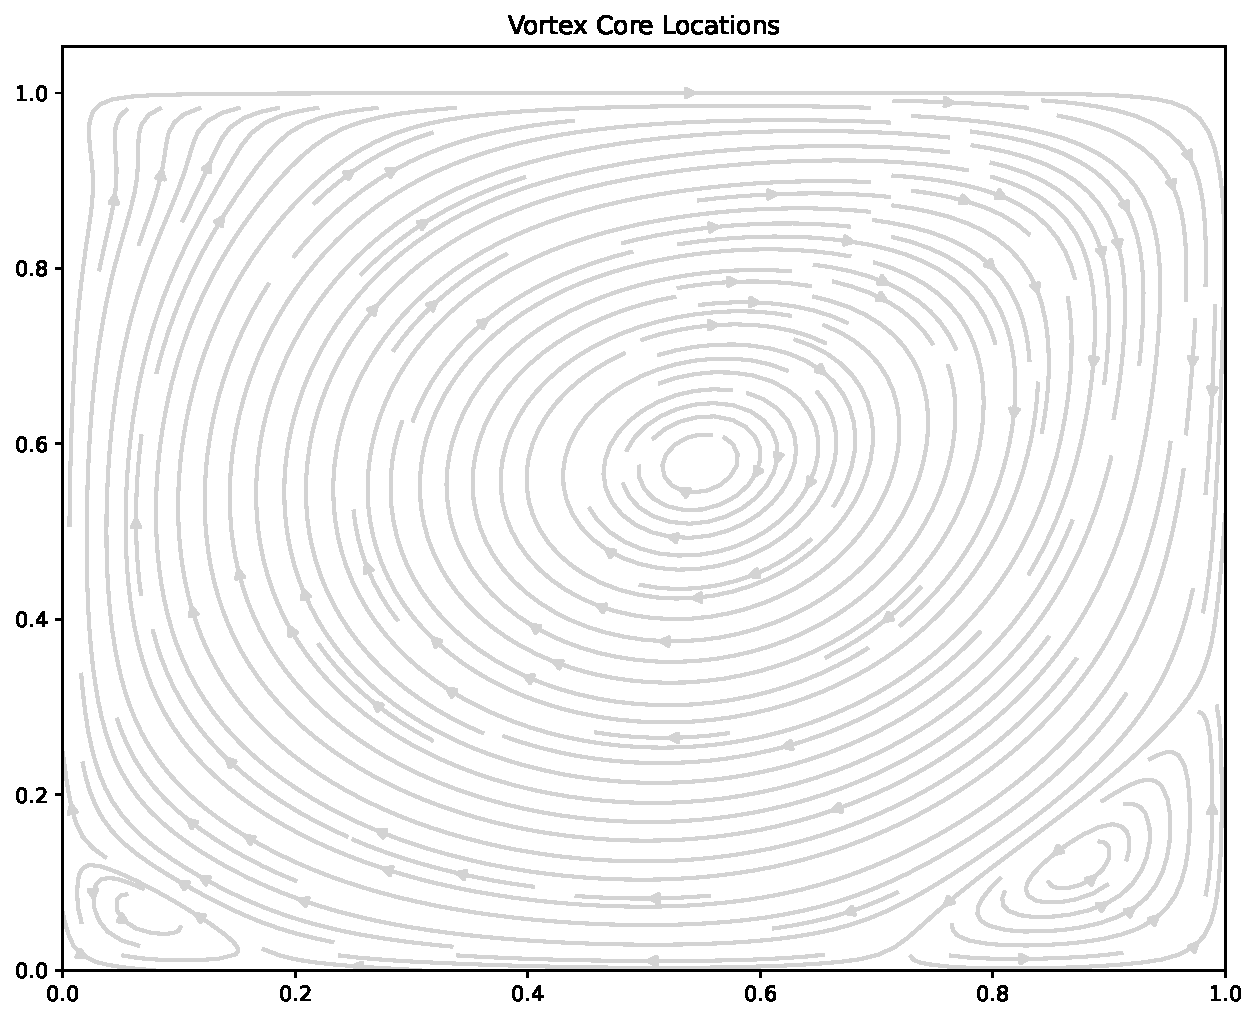
\includegraphics[width=1\textwidth]{1_streamlines.pdf}
    \caption{流线图}
    \label{fig:streamline}
\end{figure}
由流场图可以看出,主涡的涡心位置在$(0.5, 0.6)$左右,在左下角和右下角各有一个二次涡。其形成原因主要是流动边界层分离和粘性耗散效应。由于模拟条件雷诺数$Re$约等于1000,流动较为平稳,流线图中没有明显的三次涡旋结构。随着雷诺数的增加,流动会变得更加复杂,可能会出现更强的涡旋结构和不稳定性。
\begin{figure}[H]
    \centering
    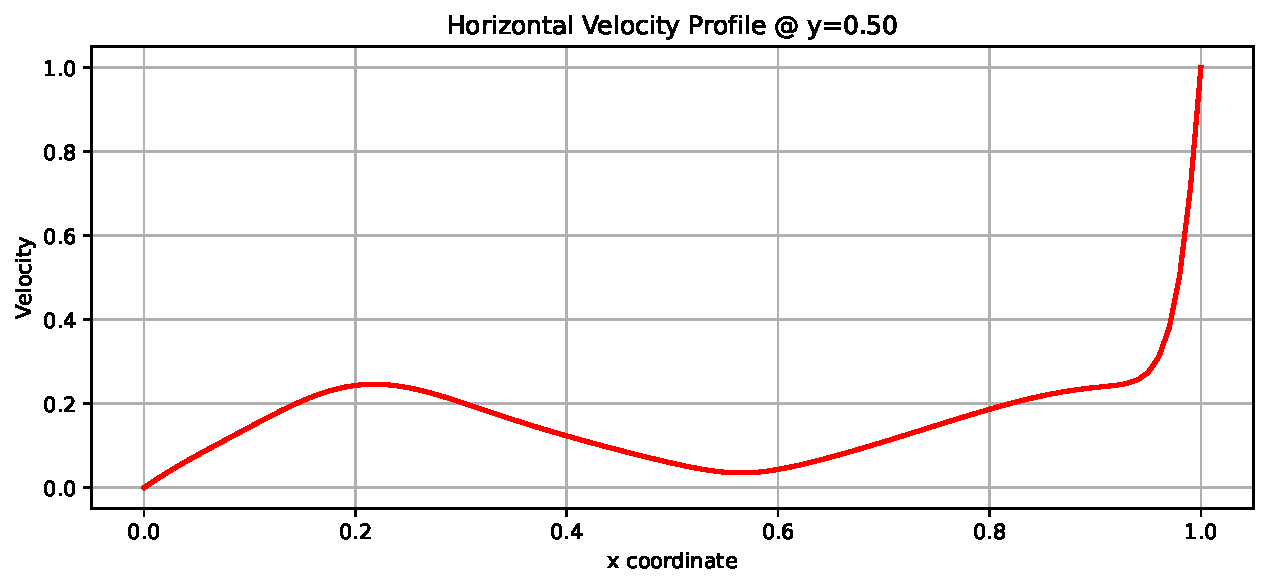
\includegraphics[width=0.8\textwidth]{2_horizontal_profile.pdf}
    \caption{y=0.5速度水平剖面图}
    \label{fig:horizontal_profile_a}
\end{figure}
\begin{figure}[H]
    \centering
    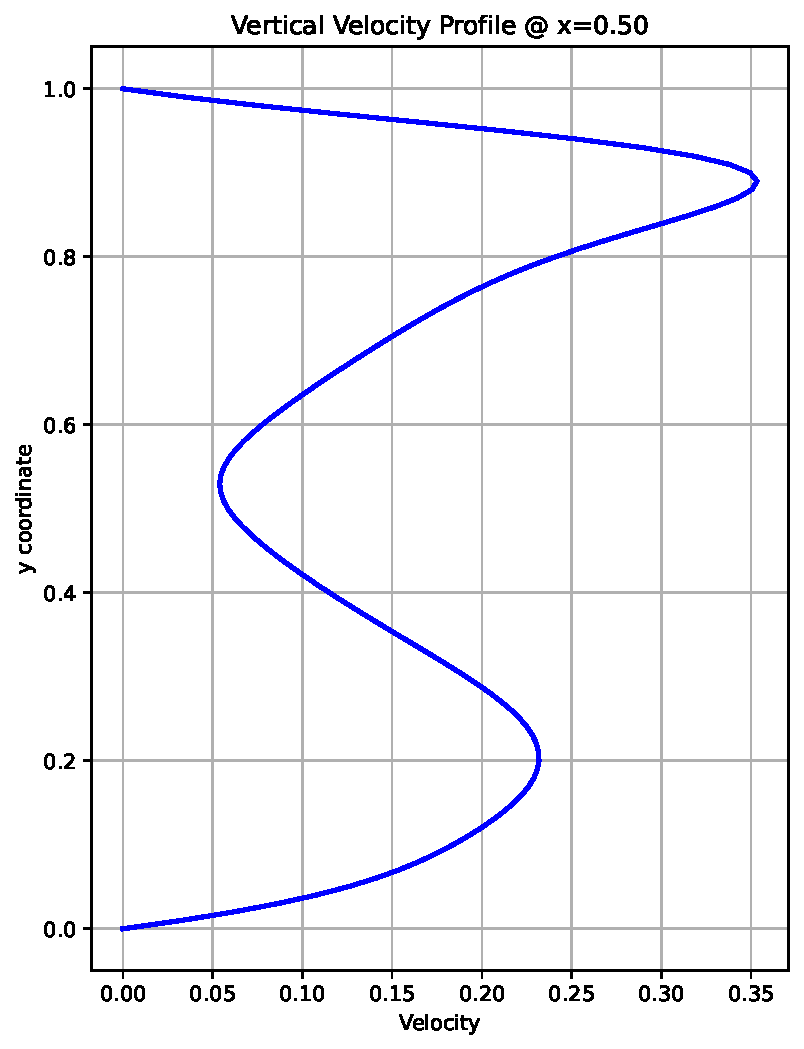
\includegraphics[width=0.6\textwidth]{3_vertical_profile.pdf}
    \caption{x=0.5速度垂直剖面图}
    \label{fig:vertical_profile_b}
\end{figure}
由速度垂直剖面图可以看出,流速在上边界处达到最大值,随着距离上边界的增加,流速减小,后增大,最后减到0。
从速度水平剖面图可以看出,流速在中间(主涡点)处达到一个极小值,左右满足边界条件为0。

\section{AI工具使用说明表}
\begin{table}[!htbp]
    \centering
    \begin{tabular}{|c|c|c|}
        \hline
        \textbf{AI名称} & \textbf{生成代码功能} & \textbf{使用内容} \\
        \hline
        Copilot & latex格式框架 & figure参数调整、图片插入\\
        \hline
        Deepseek & python绘图调整 & 68-90行图绘制的具体参数调整\\
        \hline
        Deepseek & gitignore文件忽略 & 全由ai添加\\
        \hline
\end{tabular}
\end{table}
\section{commit信息}
commit图如下:
\begin{figure}[H]
    \centering
    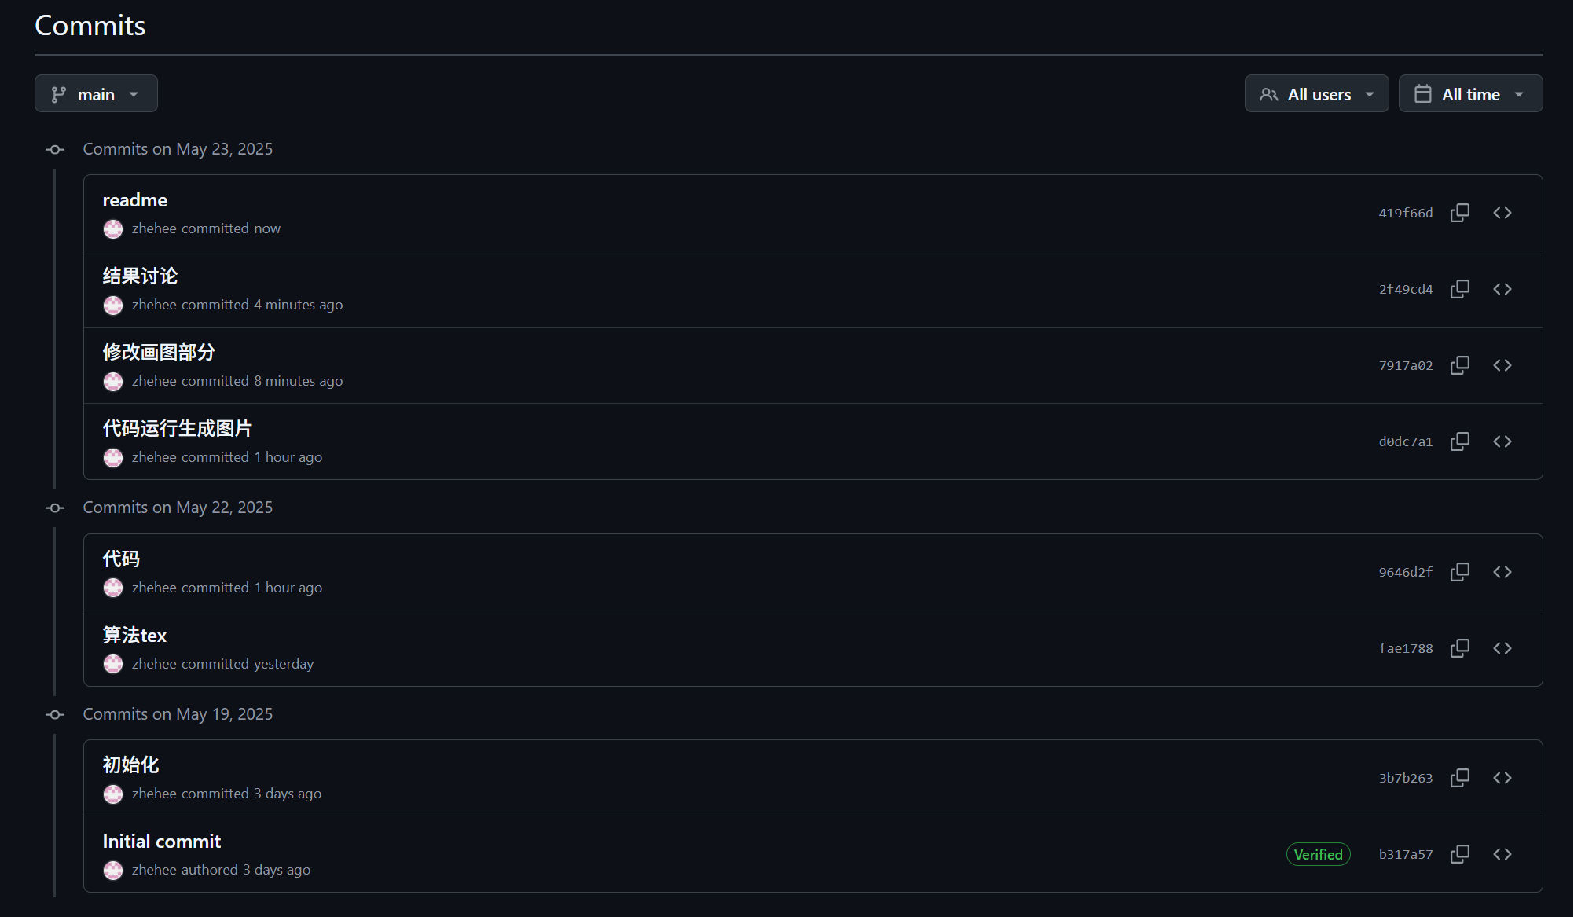
\includegraphics[width=\textwidth, height=\textheight, keepaspectratio]{commit.png}
    \caption{commits截图}
    \label{fig:commit}
\end{figure}

\end{document}